\documentclass[12pt]{article}

\usepackage{pablo}
\usepackage[a6paper,landscape,margin=.5cm]{geometry}
\pagestyle{empty}

\begin{document}

  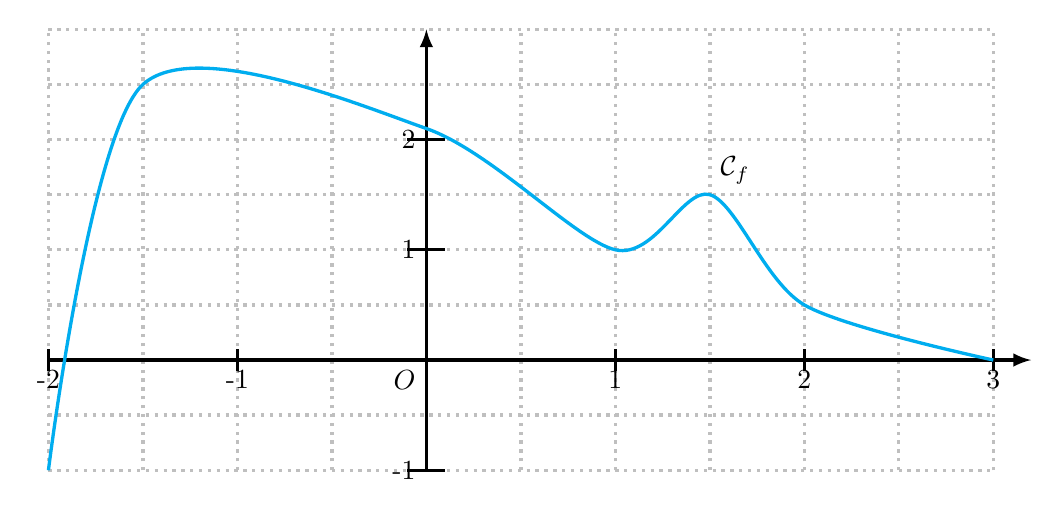
\begin{tikzpicture}[very thick,xscale=2.4, yscale=1.4]
    \draw[dotted, lightgray, xstep=.5, ystep=.5] (-2, -1) grid (3, 3);
    \draw[-latex] (-2,0) -- (3.2,0);
    \draw[-latex] (0,-1) -- (0,3);
    \foreach \x in {-2, -1, 1, 2, 3} {
      \draw (\x,0) node[below]{\x};
      \draw (\x,{0.1}) -- (\x,{-0.1});
    }
    \foreach \y in {-1, 1, 2} {
      \draw (0,\y) node[left]{\y};
      \draw (-.1, \y) -- (.1, \y);
    }
    \draw [cyan] plot [smooth, tension=0.5] coordinates {
      (-2,-1)
      (-1.5, 2.5)
      (0, 2.1)
      (1, 1)
      (1.5, 1.5)
      (2, .5)
      (3, 0)
    };
    \draw (0,0) node[below left]{$O$};
    \draw (1.5, 1.5) node[above right]{$\mathcal{C}_f$};
    %\draw (.6,3.75)  node[fill=white, opacity=.8, text opacity=1]{Altitude (m)};
    %\draw (4.5,2.25) node[fill=white, opacity=.8, text opacity=1]{Distance (km)};
  \end{tikzpicture}

  \begin{center}
    \begin{tikzpicture}[xscale=1,yscale=1]
      \tkzTabInit[lgt=1,espcl=2]
      {$x$ /1,
        $f$ /2
      }
      {-2, {-1,25}, 1, {1,5}, 3}%
    \end{tikzpicture}
  \end{center}

\end{document}
